\documentclass[11pt, letterpaper, titlepage]{article}
\usepackage[utf8]{inputenc}
\usepackage[export]{adjustbox}
\usepackage{geometry}
 \geometry{
 a4paper,
 total={168mm,257mm},
 left=20mm,
 top=15mm,
 includefoot,includehead 
 }
\usepackage[backend=biber, style=authoryear, giveninits=true, maxbibnames=25, uniquename=init, maxcitenames=2, hyperref=true, dashed=false]{biblatex}			% Benutze Biber/BibLaTeX zum Zitieren
\addbibresource{main.bib}					% Pfad zur BibTeX Datei aus Citavi
\renewcommand{\cite}{\parencite}
\usepackage{caption}
\usepackage{subcaption}
\usepackage{graphicx}
\usepackage{svg}
\usepackage{placeins}
\usepackage[hidelinks]{hyperref}
\usepackage{amsmath}
\usepackage[headsepline]{scrlayer-scrpage}
\usepackage{acronym}

\clearpairofpagestyles %Seitenzahl nicht in der Kopfzeile

\title{MeetEU Project - Team Heidelberg - Team 1 -- \\ Identification and Enhancement of novel Sars-CoV-2 NSP13 helicase inhibitors}
\author{Linda Blaier, Paul Brunner, Selina Ernst, Valerie Segatz, and Chlo\'{e} Weiler}
\date{February 2024}

\begin{document}

\maketitle

\ihead{\headmark}
\automark{section}  %Kopfzeile gleich dem Sektiontitel
\cfoot{\pagemark}   %\ofood Seitenzahl rechts

\section{Abstract}
Even though the development of vaccines against Sars-CoV-2 was successful during the recent pandemic, the amount of FDA approved drugs for the therapy of Covid-19 is still limited to Paxlovid and Veklury, Olumiant and Actemra \cite{FDA_COVID}. One possibility to accelerate the development of new therapies for Covid-19 is to screen already approved drugs for effects against the viral reproduction. In this years MeetEU project, we investigated the NSP13 helicase of Sars-CoV-2 and tried to find compounds that could be repurposed for this therapy, as well as novel compounds that could lead to an effective treatment of Covid-19. Using our \textit{in-silico} pipeline enables us to evaluate possible drug candidates, suggest novel structures based on already approved drugs and investigate their toxicity, while being cheaper and less labor intensive than projects limited to wet-lab work. 
HIER KOMMT EINE ABBILDUNG HIN


\FloatBarrier

\newpage
%    Abkürzungsverzeichnis
{\setlength{\parskip}{0.2cm}
\section*{Abbreviations}
    \begin{acronym}[LC-MS/MS23]
        % A B C D E F G H I J K L M N O P Q R S T U V W X Y Z        
        % Abkürzungen
        \acro{RTC}{replication transcription complex}
        \acro{ssRNA}{single-stranded RNA}
        \acro{DScore}{druggability score}
        \acro{MD}{Molecular dynamics}
        
        % Formelzeichen
        
        
        % als benutzt markierte Acronyme    
        
        
    \end{acronym}
}
\newpage

\section{Introduction}
General intro on nsp13 helicase... \\
In the \ac{RTC} the NSP13 helicase is present as a homodimer. Nevertheless, only one of the copies is in complex with a single-stranded RNA \ac{ssRNA}. Therefore, \textcite{Berta_2021} propose that the catalytically active form of the NSP13 helicase is the monomer \cite{Berta_2021}.  


\subsection{Identification of consensus binding pocket}
In drug discovery, the initial step is to investigate the protein structure in order to analyse potential binding sites. These are cavities on the surface or interior of the protein with suitable properties to bind a ligand. The functionality of a binding pocket is determined by its shape and location, but also by the amino acid residues which define its pyhsicochemical characteristics \cite{Stank_2016}. 
There are both different experimental and theoretical procedures existent to analyse the druggability of such binding pockets. Overall, merging distinct approaches enables a more precise prediction of the resulting consensus binding pocket which can then be further investigated using molecular docking \cite{Ricci_2022}. 

\subsection{Lead Drug Enhancement}
In order to enhance the binding affinity of our drug candidates and thus their performance, we used AutoGrow4 (Version 4.0.3) \cite{package_Autogrow4} to generate novel compounds. Starting with the best binding compounds of our initial docking simulation with AutoDock Vina as generation zero, multiple new structures are generated by combining sub-structures of the first generation or by passing them through a set of possible chemical reactions after converting them into their respective SMILES codes. All of the generated compounds are ranked by their binding affinity. After passing several filters the best performing compounds are used as the seed for the next generation. Using this algorithm, compounds are found, which show higher binding affinities than the first generation. As AutoGrow4 labels all new structures by the path by which they were obtained, we can also evaluate the synthesizability.  

\subsection{Molecular Dynamics Simulation}
As the last step of our pipeline, a MD simulation is conducted using the best scoring compounds as a ligand in the binding pocket of the NSP13 protein. Using GROMACS (Version 2023.3) \cite{package_GROMACS}, this enables us to interpret the stability of the protein-ligand interaction, as well as to identify important residues for the interaction. Using a given force-field, a set of equations describing different forces between the atoms and residues in the protein and ligand, the movement of all atoms in the system can be simulated and analysed. However, this is only possible in a very limited timeframe with a small time step size. As this process is rather resource heavy, it has to be conducted on a cluster with access to a GPU. 

\section{Material and Methods}
\subsection{Protein preparation}
In this project we analysed crystal structures of the SARS-CoV-2 NSP13 helicase which were obtained by \cite{Newman_2021} in a crystallographic fragment screening. Thus, the three protein structures (PDB codes: 6ZSL, 5RME, 5RM2) were downloaded from the protein data bank RCSB PDB. All three structures were used to obtain a consensus binding pocket. Since, 6ZSL is the crystal structure with the highest resolution of 1.94 {\AA} and both other structures show the NSP13 helicase in complex with a different fragment, we selected 6ZSL for further analysis in our drug discovery pipeline. Although the helicase is a homodimer, it was found that only the monomer is the catalytically active form. Therefore, we concentrated our drug discovery only on the monomer of the helicase, namely on chain A. \\
Protein Data Bank files often contain problems that first need to be resolved, so they can be simulated. Therefore, we prepared the PDB protein structure using the PDBFixer (Version 1.9) application, which among other things adds missing hydrogen and heavy atoms, builds missing loops and replaces non-canonical with canonical amino acids \cite{Eastman_2017}. Here, we added hydrogen atoms appropriate for the physiological pH of 7.4. Since the catalytically active form of NSP13 helicase is the monomer \cite{Berta_2021}, the additional second copy (Chain B) contained in the crystallographic structure, was removed as well as all phosphates and the ligands contained in the protein structures 5RME and 5RM2. Additionally, for molecular Docking using AutoDock Vina and for the \ac{MD} simulation the zinc ions were removed. 
For consensus binding site detection 6ZSL was used as a reference structure to align 5RME and 5RM2 in PyMol (Version 2.5.7, \textcite{PyMol_endnote}).This allowed better visualization and superimposition of the results.

\subsection{Consensus binding site detection}
To identify a potential ligand binding site of the NSP13 helicase, three different tools based on different methods were jointly used on Chain A of the crystal structures 6ZSL, 5RM2, and 5RME: (i) \textit{Fpocket} (Version 3.0, \textcite{package_Fpocket}), (ii) \textit{PrankWeb 3} (accessed on 27.12.2023, \textcite{package_P2Rank, package_PrankWeb, package_PrankWeb3}), and (iii) \textit{FTMap} (accessed on 7.12.2023, \textcite{package_FTMAP}).  
\textit{Fpocket} utilises a geometry-based algorithm based on Voronoi tessellation and sequential clustering to determine potential binding sites \cite{package_Fpocket}. Then, for each pocket different properties from the atoms of the pocket are calculated and a \ac{DScore} is assigned based on which the pockets are ranked \cite{package_Fpocket}. In this project only pockets with a \ac{DScore} above 0.2 were considered. 
We also implemented \textit{PrankWeb} \cite{package_P2Rank, package_PrankWeb, package_PrankWeb3} which is based on a machine-learning algorithm \textit{P2Rank}. It assigns structural, physico-chemical, and evolutionary features to points on the solvent accessible surface of a protein. From this information, the machine-learning model is built and used to predict and rank potential ligand binding sites based on a calculated ligandability score. It also calculates a probability for each pocket which is based on the confidence of the prediction.
The results of both tools were visualised in \textit{PyMol}. Then overlapping hot spots were merged based on the overlapping amino acid sequence and by means of visual inspection.
The third tool we used is \textit{FTMap}, which uses docking results of sixteen small molecules differing in polarity, shape and size to identify binding hot spots with a fast Fourier transform correlation. The most favorable docked confirmations are determined by energy minimization and clustering. Since there is no relatable druggability scoring function as found in both the other tools, we used \textit{FTMap} to validate the binding pocket obtained to see if indeed clusters of the small molecules formed inside the potential consensus binding pocket.
Lastly, the coordinates of the consensus binding pocket needed for molecular docking were calculated using the public server at usegalaxy.org of the Galaxy web platform \cite{galaxy}. The docking box size was set to $30 {\AA}^3$ to ensure that all amino acids that of the pocket that could potentially interact with a ligand and that larger ligands are included in the molecular docking simulation.

\section{Results} 
\subsection{Consensus binding site detection}
Before we could screen ligand libraries for potential inhibitorrs, the druggability of the surface of the NSP13 helicase needed to be investigated to determine ligand binding sites. For a more precise identification three different crystal structures (PDB codes: 6ZSL, 5RM2, 5RME) were analysed using three different tools which follow distinct computational methods. The calculated binding hot spots were visualised in PyMol \cite{PyMol_endnote} and overlapping ones were merged through visual examination to obtain a consensus binding site.
Overall, the hot spots calculated with Fpocket which overlapped between the three crystal structures all ranked first among the calculated binding sites for each crystal structure. Their \acp{DScore} were 0.647 for 6ZSL, 0.383 for 5RM2, and 0.875 for 5RME. Also, the respective overlapping binding sites calculated with PrankWeb ranked either first (5RM2 and 5RME) or second (6ZSL) among the calculated binding sites. Therefore, the respective Scores and calculated Probability was also among the highest for these binding sites (Score of 9.69 and Probability of 0.562 for 6ZSL, Score of 22.15 and Probability of 0.860 for 5RM2, and a Score of 17.91 and a Probability of 0809 for 5RME). Additionally, four other hot spots detected for 6ZSL and 5RME which contained some overlapping amino acids with the highest ranked pockets were merged into the consensus binding pocket. But these, were ranked lower by PrankWeb and also contained additional amino acids not present in the highest ranked binding sites. 
Interestingly, for the crystal structure 5RME a second binding hot spot was detected in proximity to the 1B domain. Nevertheless, because this binding site was only found in one crystal structure and the underlying pockets were ranked very low by both Fpocket and PrankWeb, this binding site was not considered for further analysis.
The resulting consensus binding pocket is located in the ATP binding pocket in between the two RecA-like domains A1 and A2 (Figure \ref{consensus_binding_pocket}). 
\begin{figure}
    \centering
    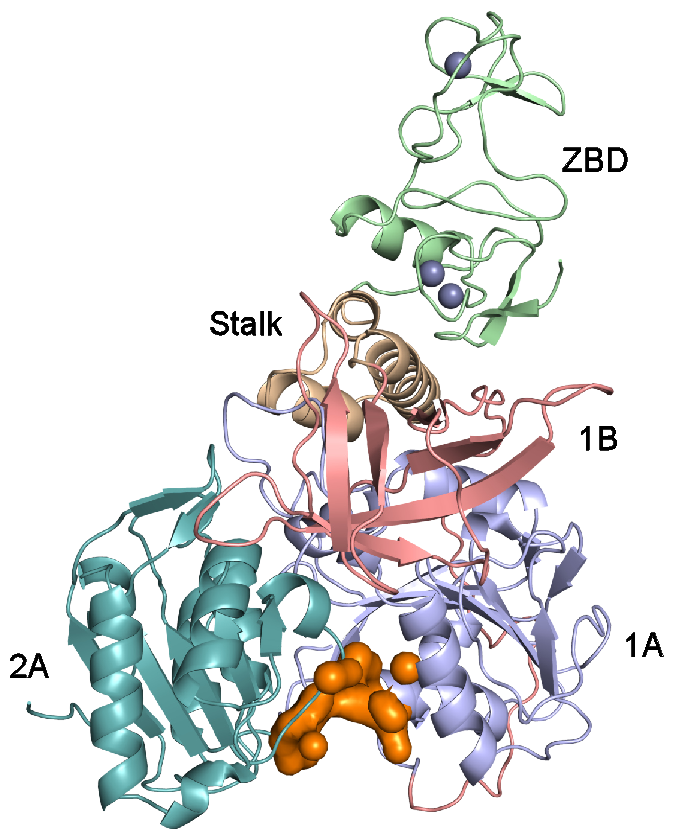
\includegraphics[width=0.6\textwidth]{consens_domain_big.pdf}
    \caption{Consensus binding pocket of the NSP13 helicase. The binding pocket is located in the ATP binding pocket in between the two RecA-like domains A1 and A2.}
    \label{consensus_binding_pocket}
\end{figure}

\FloatBarrier

\section{Discussion and Outlook}

\section{Supplementary Material}

\pagebreak
\FloatBarrier

\renewcommand{\bibname}{References}  % damit Literatuverzeicnis mit "References" betitelt
\printbibliography

\end{document}
